\documentclass[12pt,a4paper]{article}

% ─── Page Layout ───────────────────────────────────────────────────────────────
\usepackage[a4paper, margin=0.8in, headheight=14pt]{geometry}

% ─── Fonts (XeLaTeX) ───────────────────────────────────────────────────────────
\usepackage{fontspec}
\usepackage{unicode-math}
\setmainfont{TeX Gyre Pagella}
\setmonofont[Scale=0.88]{TeX Gyre Cursor}
\setmathfont{Latin Modern Math}

% ─── Packages ──────────────────────────────────────────────────────────────────
\usepackage{xcolor}
\usepackage{colortbl}
\usepackage{titlesec}
\usepackage{enumitem}
\usepackage{tabularx}
\usepackage{booktabs}
\usepackage{array}
\usepackage{amsmath}
\usepackage{tikz}
\usetikzlibrary{shapes.geometric, arrows.meta, positioning, calc, fit, decorations.pathreplacing, patterns}
\usepackage{tcolorbox}
\tcbuselibrary{skins, breakable}
\usepackage{hyperref}
\usepackage{fancyhdr}
\usepackage{graphicx}
\usepackage{microtype}
\hyphenpenalty=10000
\exhyphenpenalty=10000
\sloppy
\usepackage{caption}
\usepackage{setspace}
\usepackage{multirow}
\usepackage{tocloft}

% ─── Q&A helper ────────────────────────────────────────────────────────────────
\newcommand{\Q}[1]{\textbf{#1}\par\noindent\ignorespaces}

% ─── Colour Palette ────────────────────────────────────────────────────────────
\definecolor{myred}{RGB}{196,30,58}
\definecolor{mydark}{RGB}{30,30,50}
\definecolor{mygreen}{RGB}{14,120,80}
\definecolor{myteal}{RGB}{0,130,140}
\definecolor{myamber}{RGB}{180,100,0}
\definecolor{mypurple}{RGB}{100,30,160}
\definecolor{mygray}{RGB}{246,247,249}
\definecolor{mgframe}{RGB}{180,185,200}
\definecolor{watermark}{RGB}{145,150,170}
\definecolor{hdrred}{RGB}{250,232,235}
\definecolor{hdrgreen}{RGB}{220,244,233}
\definecolor{hdrteal}{RGB}{220,242,244}
\definecolor{hdramber}{RGB}{253,242,215}
\definecolor{hdrpurple}{RGB}{238,228,255}
\definecolor{hdrgray}{RGB}{238,240,245}
\definecolor{rowalt}{RGB}{250,251,253}

% ─── Section Formatting ────────────────────────────────────────────────────────
\titleformat{\section}
  {\large\bfseries\color{myred}}{\thesection.}{0.5em}{}
  [\vspace{1pt}{\color{myred}\rule{\linewidth}{0.8pt}}]
\titleformat{\subsection}
  {\normalsize\bfseries\color{myteal}}{\thesubsection}{0.5em}{}
\titlespacing*{\section}{0pt}{18pt}{7pt}
\titlespacing*{\subsection}{0pt}{11pt}{4pt}

% ─── Paragraph ─────────────────────────────────────────────────────────────────
\setlength{\parindent}{0pt}
\setlength{\parskip}{4pt}

% ─── TOC Styling ───────────────────────────────────────────────────────────────
\renewcommand{\cfttoctitlefont}{\large\bfseries\color{myred}}
\renewcommand{\cftaftertoctitle}{\par\noindent{\color{myred}\rule{\linewidth}{0.8pt}}}
\setlength{\cftbeforetoctitleskip}{0pt}
\setlength{\cftaftertoctitleskip}{6pt}
\renewcommand{\cftsecfont}{\normalsize\bfseries\color{mydark}}
\renewcommand{\cftsecpagefont}{\normalsize\bfseries\color{mydark}}
\renewcommand{\cftsecleader}{\cftdotfill{\cftdotsep}}
\setlength{\cftbeforesecskip}{7pt}
\renewcommand{\cftsubsecfont}{\small\color{mydark}}
\renewcommand{\cftsubsecpagefont}{\small\color{mydark}}
\setlength{\cftbeforesubsecskip}{3pt}
\setlength{\cftsubsecindent}{1.4em}

% ─── Table helpers ─────────────────────────────────────────────────────────────
\renewcommand{\arraystretch}{1.45}
\setlength{\tabcolsep}{6pt}
\arrayrulecolor{mydark}
\newcolumntype{B}[1]{>{\small\bfseries\raggedright\arraybackslash}m{#1}}
\newcolumntype{Y}{>{\small\raggedright\arraybackslash}X}
\renewcommand{\tabularxcolumn}[1]{m{#1}}

% ─── Header / Footer ───────────────────────────────────────────────────────────
\pagestyle{fancy}
\fancyhf{}
\fancyhead[L]{\small\color{myred}\textbf{BS-M301}\;\color{mydark}--- Probability and Statistics}
\fancyhead[R]{\small\color{myteal}\textbf{Module 6 Notes}}
\fancyfoot[C]{\small\color{mydark}\thepage}
\fancyfoot[R]{\small\color{watermark}\textit{\copyright\ Biraj}}
\renewcommand{\headrulewidth}{0.5pt}
\renewcommand{\footrulewidth}{0.3pt}

% ─── Hyperref ──────────────────────────────────────────────────────────────────
\hypersetup{
  colorlinks=true, linkcolor=myteal, urlcolor=myteal,
  pdfauthor={Biraj Sarkar (CGEC)},
  pdftitle={BS-M301 --- Module 6 Notes: Small Samples}
}

% ─── tcolorbox styles ──────────────────────────────────────────────────────────
\tcbset{
  tikzbox/.style={
    colback=mygray, colframe=mgframe, boxrule=0.6pt, arc=4pt,
    left=8pt, right=8pt, top=6pt, bottom=6pt,
    colbacktitle=mgframe, coltitle=mydark,
    fonttitle=\small\bfseries
  },
  defbox/.style={
    colback=hdrgreen, colframe=mygreen, boxrule=0.8pt, arc=4pt,
    left=9pt, right=9pt, top=6pt, bottom=6pt,
    colbacktitle=mygreen, coltitle=white,
    fonttitle=\small\bfseries
  },
  formulabox/.style={
    colback=hdrteal, colframe=myteal, boxrule=0.8pt, arc=4pt,
    left=9pt, right=9pt, top=7pt, bottom=7pt,
    colbacktitle=myteal, coltitle=white,
    fonttitle=\small\bfseries
  },
  examplebox/.style={
    colback=hdramber, colframe=myamber, boxrule=0.8pt, arc=4pt,
    left=9pt, right=9pt, top=6pt, bottom=6pt,
    colbacktitle=myamber, coltitle=white,
    fonttitle=\small\bfseries
  },
  masonbox/.style={
    colback=hdrpurple, colframe=mypurple, boxrule=0.8pt, arc=4pt,
    left=9pt, right=9pt, top=6pt, bottom=6pt,
    colbacktitle=mypurple, coltitle=white,
    fonttitle=\small\bfseries
  },
  exambox/.style={
    colback=hdrpurple, colframe=mypurple, boxrule=1pt, arc=5pt,
    left=10pt, right=10pt, top=8pt, bottom=8pt,
    colbacktitle=mypurple, coltitle=white,
    fonttitle=\bfseries,
    breakable, title after break={\textbf{Frequently Asked / Viva Questions (contd.)}}
  }
}
\tcbset{breakable}
\tcbset{after={\color{black}}}

% ─── TikZ styles ───────────────────────────────────────────────────────────────
\tikzset{
  arrow/.style={-Stealth, thick, color=mydark},
  redarrow/.style={-Stealth, thick, color=myred},
  line/.style={thick, color=mydark}
}

\begin{document}

% ─── Title Page ────────────────────────────────────────────────────────────────
\begin{center}
  {\Large\bfseries\color{myred} BS-M301 --- PROBABILITY AND STATISTICS}\\[4pt]
  {\large\bfseries\color{myteal} MODULE 6: SMALL SAMPLES}\\[4pt]
  {\small\color{mydark}\textbf{B.Tech ECE --- 3rd Semester} \;\vert\; MAKAUT Syllabus: 4L}\\[2pt]
  {\footnotesize\color{watermark} Author: Biraj Sarkar (CGEC) \;\vert\; Typeset in XeLaTeX}
\end{center}
\noindent{\color{myred}\rule{\linewidth}{1.2pt}}
\vspace{6pt}

\tableofcontents
\vspace{10pt}
\noindent{\color{mgframe}\rule{\linewidth}{0.5pt}}
\vspace{8pt}

% ===============================================================================
\section{Introduction to Small Sample Theory}
% ===============================================================================

\begin{tcolorbox}[defbox, title={\textbf{Definition: Small Samples vs. Large Samples}}]
In statistical hypothesis testing, a sample is designated as a \textbf{small sample} if its sample size $n < 30$.
\begin{itemize}[leftmargin=12pt, itemsep=2pt]
  \item \textbf{Large Samples ($n \ge 30$):} By the Central Limit Theorem (CLT), the sampling distribution of sample means approaches normality regardless of the parent distribution. The sample standard deviation $s$ closely approximates the population standard deviation $\sigma$, justifying the use of the standard normal $Z$-test.
  \item \textbf{Small Samples ($n < 30$):} The CLT cannot be invoked. The parent population \textbf{must be assumed normally distributed}. Furthermore, replacing $\sigma$ with the sample variance $s^2 = \frac{1}{n-1}\sum (x_i - \bar{x})^2$ introduces substantial additional sampling fluctuations, yielding distributions with heavier tails than $N(0, 1)$.
\end{itemize}
Hence, small sample inference relies on the \textbf{exact sampling distributions}:
\begin{enumerate}[leftmargin=16pt, itemsep=1pt]
  \item \textbf{Student's $t$-distribution} (W.~S.~Gosset, 1908): For inference on population means and correlation coefficients when $\sigma$ is unknown.
  \item \textbf{Snedecor's $F$-distribution} (G.~W.~Snedecor \& R.~A.~Fisher): For testing the ratio of two independent population variances.
  \item \textbf{Chi-square ($\chi^2$) distribution} (Karl Pearson, 1900): For tests of goodness of fit and independence of attributes in contingency tables.
\end{enumerate}
\end{tcolorbox}

\begin{tcolorbox}[formulabox, title={\textbf{Degrees of Freedom ($\nu$ or d.f.)}}]
The \textbf{degrees of freedom} ($\nu$) of a test statistic represents the number of unconstrained, freely variable observations available in the calculation:
\begin{equation}
  \nu = n - k
\end{equation}
where $n$ is the total number of sample observations and $k$ is the number of linear constraints or sample-derived parameters estimated to compute the statistic (e.g., estimating $\mu$ by $\bar{x}$ consumes 1 d.f., so $\nu = n - 1$).
\end{tcolorbox}

% ===============================================================================
\section{Student's \texorpdfstring{$t$}{t}-Distribution}
% ===============================================================================

\subsection{Definition and Derivation}

\begin{tcolorbox}[defbox, title={\textbf{Mathematical Definition of Student's $t$-Variable}}]
Let $Z \sim N(0, 1)$ be a standard normal random variable, and let $Y \sim \chi^2(\nu)$ be an independent Chi-square random variable with $\nu$ degrees of freedom. The ratio:
\begin{equation}
  T = \frac{Z}{\sqrt{\dfrac{Y}{\nu}}}
\end{equation}
follows \textbf{Student's $t$-distribution} with $\nu$ degrees of freedom, written $T \sim t(\nu)$.
\end{tcolorbox}

\subsection{Probability Density Function and Properties}

The probability density function (PDF) of $T \sim t(\nu)$ is:
\begin{equation}
  f(t) = \frac{1}{\sqrt{\nu}\,\mathrm{B}\left(\dfrac{1}{2}, \dfrac{\nu}{2}\right)}\left(1 + \frac{t^2}{\nu}\right)^{-\frac{\nu+1}{2}}, \quad -\infty < t < \infty
\end{equation}
where $\mathrm{B}\left(\frac{1}{2}, \frac{\nu}{2}\right) = \frac{\sqrt{\pi}\,\Gamma(\nu/2)}{\Gamma((\nu+1)/2)}$ is the Beta function.

\begin{tcolorbox}[formulabox, title={\textbf{Key Properties of Student's $t$-Distribution}}]
\begin{enumerate}[leftmargin=14pt, itemsep=2pt]
  \item \textbf{Symmetry:} The curve is bell-shaped and symmetric about $t = 0$. All odd central moments are zero:
  \begin{equation}
    \mu_{2k+1} = E[T^{2k+1}] = 0 \quad (\text{for } \nu > 2k+1)
  \end{equation}
  \item \textbf{Mean:} $\mu_1' = E[T] = 0$ (valid for $\nu > 1$).
  \item \textbf{Variance:} $\mathrm{Var}(T) = \mu_2 = \dfrac{\nu}{\nu - 2}$ (valid for $\nu > 2$). Note that $\mathrm{Var}(T) > 1$.
  \item \textbf{Kurtosis (Heavy Tails):} The distribution is leptokurtic ($\beta_2 > 3$). For $\nu > 4$:
  \begin{equation}
    \beta_2 = \frac{\mu_4}{\mu_2^2} = 3 + \frac{6}{\nu - 4} > 3
  \end{equation}
  \item \textbf{Limiting Form (Asymptotic Normality):} As $\nu \to \infty$, the $t$-distribution converges to the standard normal distribution:
  \begin{equation}
    \lim_{\nu \to \infty} \left(1 + \frac{t^2}{\nu}\right)^{-\frac{\nu+1}{2}} = e^{-t^2/2} \implies t(\nu) \xrightarrow{d} N(0, 1)
  \end{equation}
\end{enumerate}
\end{tcolorbox}

\begin{tcolorbox}[tikzbox, title={\textbf{TikZ Illustration: Comparison of Student's $t$ vs. Standard Normal $N(0, 1)$}}]
\centering
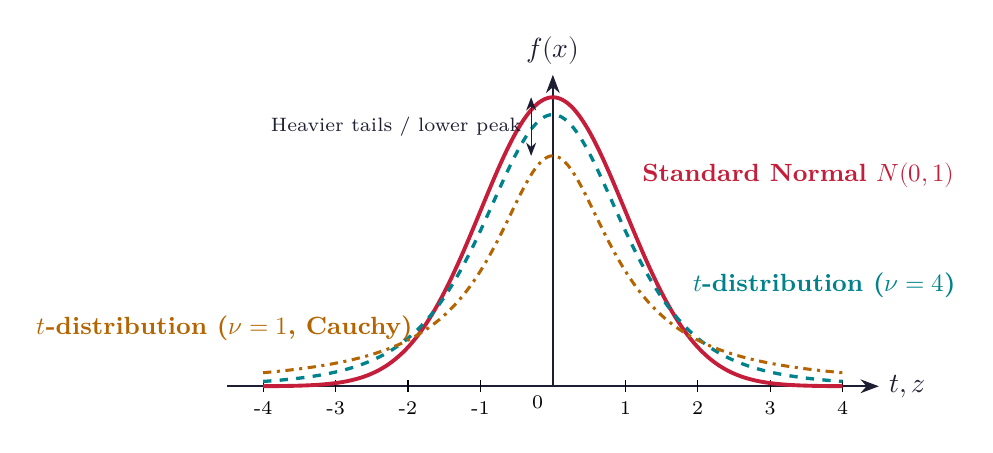
\begin{tikzpicture}[scale=0.92]
  \draw[arrow] (-4.5, 0) -- (4.5, 0) node[right] {$t, z$};
  \draw[arrow] (0, 0) -- (0, 4.3) node[above] {$f(x)$};

  \foreach \x in {-4, -3, -2, -1, 1, 2, 3, 4}
    \draw (\x, 0.08) -- (\x, -0.08) node[below, font=\scriptsize] {\x};
  \node[below left, font=\scriptsize] at (0, 0) {$0$};

  % Normal curve N(0,1): f(0) = 0.3989 -> 3.99 cm
  \draw[line width=1.4pt, color=myred, domain=-4:4, samples=100, smooth]
    plot (\x, {3.989 * exp(-\x*\x / 2)});
  \node[color=myred, font=\small\bfseries, above right] at (1.1, 2.6) {Standard Normal $N(0, 1)$};

  % Student's t, nu = 4: f(0) = 0.375 -> 3.75 cm
  \draw[line width=1.2pt, color=myteal, dashed, domain=-4:4, samples=100, smooth]
    plot (\x, {3.75 * (1 + \x*\x / 4)^(-2.5)});
  \node[color=myteal, font=\small\bfseries, right] at (1.8, 1.4) {$t$-distribution ($\nu = 4$)};

  % Student's t, nu = 1 (Cauchy): f(0) = 1/pi -> 3.18 cm
  \draw[line width=1.1pt, color=myamber, dashdotted, domain=-4:4, samples=100, smooth]
    plot (\x, {3.183 / (1 + \x*\x)});
  \node[color=myamber, font=\small\bfseries, left] at (-1.8, 0.8) {$t$-distribution ($\nu = 1$, Cauchy)};

  % Heavier tails annotation
  \draw[<->, >=Stealth, color=mydark] (-0.3, 3.18) -- (-0.3, 3.99) node[midway, left, font=\scriptsize] {Heavier tails / lower peak};
\end{tikzpicture}
\end{tcolorbox}

\newpage
% ===============================================================================
\section{Student's \texorpdfstring{$t$}{t}-Tests of Significance}
% ===============================================================================

\subsection{Test for Single Mean}

\begin{tcolorbox}[formulabox, title={\textbf{Test 1: Single Mean $t$-Test Formulation}}]
Let $x_1, x_2, \ldots, x_n$ be a random sample of size $n < 30$ drawn from a normal population $N(\mu, \sigma^2)$ where $\sigma$ is unknown. We test:
\begin{equation}
  H_0: \mu = \mu_0 \quad \text{vs.} \quad H_1: \mu \ne \mu_0 \quad (\text{or one-sided } \mu > \mu_0, \mu < \mu_0)
\end{equation}
The test statistic is:
\begin{equation}
  t = \frac{\bar{x} - \mu_0}{s / \sqrt{n}}
\end{equation}
where $\bar{x} = \frac{1}{n}\sum_{i=1}^n x_i$ and the \textbf{unbiased sample variance} is:
\begin{equation}
  s^2 = \frac{1}{n - 1} \sum_{i=1}^n (x_i - \bar{x})^2 = \frac{1}{n - 1}\left(\sum_{i=1}^n x_i^2 - \frac{(\sum x_i)^2}{n}\right)
\end{equation}
Under $H_0$, $t \sim t(\nu)$ with degrees of freedom $\nu = n - 1$.

\textbf{Decision Rule (Two-tailed at significance level $\alpha$):}
\begin{itemize}[leftmargin=12pt, itemsep=2pt]
  \item Reject $H_0$ if $|t_{\text{cal}}| > t_{\alpha/2, n-1}$.
  \item Fail to reject $H_0$ if $|t_{\text{cal}}| \le t_{\alpha/2, n-1}$.
\end{itemize}
\textbf{$100(1-\alpha)\%$ Confidence Interval for $\mu$:}
\begin{equation}
  \bar{x} - t_{\alpha/2, n-1} \frac{s}{\sqrt{n}} \le \mu \le \bar{x} + t_{\alpha/2, n-1} \frac{s}{\sqrt{n}}
\end{equation}
\end{tcolorbox}

\begin{tcolorbox}[examplebox, title={\textbf{Worked Example: Single Mean $t$-Test}}]
A manufacturer claims that the mean lifetime of an electronic component is 1000 hours. A random sample of 9 components yields a sample mean of 980 hours with a sample standard deviation $s = 30$ hours. Test at the 5\% level whether the true mean lifetime is significantly less than 1000 hours ($t_{0.05, 8} = 1.860$).

\textbf{Solution:}
\begin{enumerate}[leftmargin=14pt, itemsep=2pt]
  \item \textbf{Hypotheses:} $H_0: \mu = 1000$ vs. $H_1: \mu < 1000$ (one-tailed left-sided test).
  \item \textbf{Parameters:} $n = 9$, $\bar{x} = 980$, $s = 30$, $\mu_0 = 1000$.
  \item \textbf{Test Statistic:}
  \begin{equation*}
    t_{\text{cal}} = \frac{\bar{x} - \mu_0}{s / \sqrt{n}} = \frac{980 - 1000}{30 / \sqrt{9}} = \frac{-20}{10} = -2.00
  \end{equation*}
  \item \textbf{Critical Value:} For left-tailed test at $\alpha = 0.05$ with $\nu = 8$: $t_{\text{crit}} = -1.860$.
  \item \textbf{Conclusion:} Since $t_{\text{cal}} = -2.00 < -1.860$, $t_{\text{cal}}$ falls in the critical rejection region. We reject $H_0$ and conclude that the mean lifetime is significantly less than 1000 hours.
\end{enumerate}
\end{tcolorbox}

\subsection{Test for Difference of Two Means (Independent Samples)}

\begin{tcolorbox}[formulabox, title={\textbf{Test 2: Two-Sample Independent $t$-Test with Pooled Variance}}]
Let two independent samples of sizes $n_1$ and $n_2$ be drawn from normal populations $N(\mu_1, \sigma^2)$ and $N(\mu_2, \sigma^2)$ with \textbf{equal unknown variance} ($\sigma_1^2 = \sigma_2^2 = \sigma^2$). We test:
\begin{equation}
  H_0: \mu_1 = \mu_2 \quad \text{vs.} \quad H_1: \mu_1 \ne \mu_2
\end{equation}
The \textbf{pooled unbiased variance} $s_p^2$ combining both samples is:
\begin{equation}
  s_p^2 = \frac{\sum_{i=1}^{n_1} (x_{1i} - \bar{x}_1)^2 + \sum_{j=1}^{n_2} (x_{2j} - \bar{x}_2)^2}{n_1 + n_2 - 2} = \frac{(n_1 - 1)s_1^2 + (n_2 - 1)s_2^2}{n_1 + n_2 - 2}
\end{equation}
The test statistic is:
\begin{equation}
  t = \frac{\bar{x}_1 - \bar{x}_2}{s_p \sqrt{\dfrac{1}{n_1} + \dfrac{1}{n_2}}}
\end{equation}
Under $H_0$, $t \sim t(\nu)$ with degrees of freedom $\nu = n_1 + n_2 - 2$.
\end{tcolorbox}

\subsection{Paired \texorpdfstring{$t$}{t}-Test for Dependent Samples}

\begin{tcolorbox}[defbox, title={\textbf{Test 3: Paired $t$-Test Principle}}]
When observations in two samples are drawn in matched pairs (e.g., measurements taken on the \textbf{same physical circuit before and after} temperature cycling), the two groups are statistically dependent. We eliminate inter-subject variability by evaluating individual differences:
\begin{equation}
  d_i = x_i - y_i, \quad i = 1, 2, \ldots, n
\end{equation}
Under the null hypothesis of no treatment effect ($H_0: \mu_d = 0$):
\begin{equation}
  t = \frac{\bar{d} - 0}{s_d / \sqrt{n}}
\end{equation}
where:
\begin{equation}
  \bar{d} = \frac{1}{n}\sum_{i=1}^n d_i, \qquad s_d^2 = \frac{1}{n - 1}\sum_{i=1}^n (d_i - \bar{d})^2 = \frac{\sum d_i^2 - \dfrac{(\sum d_i)^2}{n}}{n - 1}
\end{equation}
The statistic follows Student's $t$-distribution with $\nu = n - 1$ degrees of freedom.
\end{tcolorbox}

\subsection{Test for Significance of Correlation Coefficient}

\begin{tcolorbox}[formulabox, title={\textbf{Test 4: Significance of Correlation Coefficient}}]
Let $r$ be the Pearson sample correlation coefficient calculated from $n$ pairs of observations drawn from a bivariate normal population. To test:
\begin{equation}
  H_0: \rho = 0 \quad (\text{variables are uncorrelated}) \quad \text{vs.} \quad H_1: \rho \ne 0
\end{equation}
The test statistic is:
\begin{equation}
  t = \frac{r \sqrt{n - 2}}{\sqrt{1 - r^2}}
\end{equation}
Under $H_0$, $t \sim t(\nu)$ with degrees of freedom $\nu = n - 2$. Reject $H_0$ if $|t_{\text{cal}}| > t_{\alpha/2, n-2}$.
\end{tcolorbox}

\newpage
% ===============================================================================
\section{Snedecor's \texorpdfstring{$F$}{F}-Distribution and Test for Ratio of Variances}
% ===============================================================================

\subsection{Definition and Properties}

\begin{tcolorbox}[defbox, title={\textbf{Definition of Snedecor's $F$-Distribution}}]
Let $U \sim \chi^2(\nu_1)$ and $V \sim \chi^2(\nu_2)$ be two independent Chi-square random variables with $\nu_1$ and $\nu_2$ degrees of freedom, respectively. The ratio:
\begin{equation}
  F = \frac{U / \nu_1}{V / \nu_2}
\end{equation}
follows \textbf{Snedecor's $F$-distribution} with $(\nu_1, \nu_2)$ degrees of freedom, denoted $F \sim F(\nu_1, \nu_2)$.
\end{tcolorbox}

\begin{tcolorbox}[formulabox, title={\textbf{Properties of the $F$-Distribution}}]
\begin{enumerate}[leftmargin=14pt, itemsep=2pt]
  \item \textbf{Support and Shape:} $F \in (0, \infty)$. The distribution is positively skewed (right-skewed) and unimodal.
  \item \textbf{Mean:} $E[F] = \dfrac{\nu_2}{\nu_2 - 2}$ (for $\nu_2 > 2$, independent of $\nu_1$).
  \item \textbf{Variance:} $\mathrm{Var}(F) = \dfrac{2\nu_2^2(\nu_1 + \nu_2 - 2)}{\nu_1(\nu_2 - 2)^2(\nu_2 - 4)}$ (for $\nu_2 > 4$).
  \item \textbf{Reciprocal Property:} If $F \sim F(\nu_1, \nu_2)$, then $\dfrac{1}{F} \sim F(\nu_2, \nu_1)$. Hence:
  \begin{equation}
    F_{1-\alpha, \nu_1, \nu_2} = \frac{1}{F_{\alpha, \nu_2, \nu_1}}
  \end{equation}
  \item \textbf{Relation to $t$ and $\chi^2$:}
  \begin{equation}
    F_{1, \nu} = t_\nu^2, \qquad \lim_{\nu_2 \to \infty} \nu_1 F_{\nu_1, \nu_2} = \chi^2(\nu_1)
  \end{equation}
\end{enumerate}
\end{tcolorbox}

\subsection{\texorpdfstring{$F$}{F}-Test for Equality of Two Population Variances}

\begin{tcolorbox}[formulabox, title={\textbf{$F$-Test Procedure for $\sigma_1^2 = \sigma_2^2$}}]
Let two independent random samples of sizes $n_1$ and $n_2$ be drawn from normal populations $N(\mu_1, \sigma_1^2)$ and $N(\mu_2, \sigma_2^2)$. We test:
\begin{equation}
  H_0: \sigma_1^2 = \sigma_2^2 \quad \text{vs.} \quad H_1: \sigma_1^2 \ne \sigma_2^2 \quad (\text{or } \sigma_1^2 > \sigma_2^2)
\end{equation}
Compute the unbiased sample variances:
\begin{equation}
  s_1^2 = \frac{1}{n_1 - 1}\sum_{i=1}^{n_1} (x_{1i} - \bar{x}_1)^2, \qquad s_2^2 = \frac{1}{n_2 - 1}\sum_{j=1}^{n_2} (x_{2j} - \bar{x}_2)^2
\end{equation}
By convention, we place the larger sample variance in the numerator:
\begin{equation}
  F_{\text{cal}} = \frac{s_1^2}{s_2^2} \ge 1 \quad (\text{assuming } s_1^2 \ge s_2^2)
\end{equation}
with degrees of freedom $\nu_1 = n_1 - 1$ (numerator) and $\nu_2 = n_2 - 1$ (denominator). Reject $H_0$ at level $\alpha$ if $F_{\text{cal}} > F_{\alpha/2, \nu_1, \nu_2}$.
\end{tcolorbox}

\begin{tcolorbox}[tikzbox, title={\textbf{TikZ Schematic: Right-Skewed $F$-Distribution with Critical Region}}]
\centering
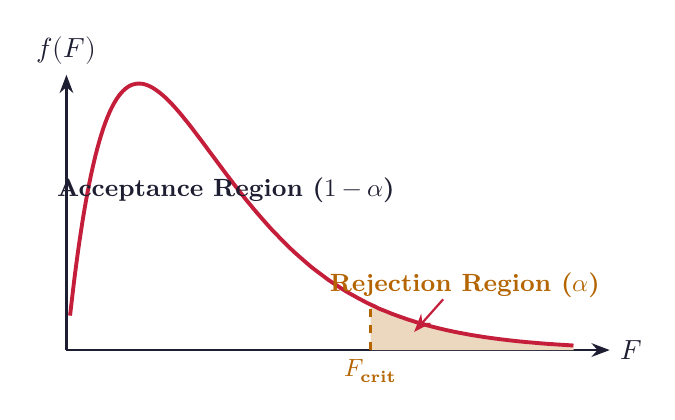
\begin{tikzpicture}[scale=0.92]
  \draw[arrow] (0, 0) -- (7.5, 0) node[right] {$F$};
  \draw[arrow] (0, 0) -- (0, 3.8) node[above] {$f(F)$};

  % Shaded rejection region
  \fill[myamber!25] plot[domain=4.2:7, samples=50] (\x, {10 * \x * exp(-\x)}) -- (7, 0) -- (4.2, 0) -- cycle;

  % F curve
  \draw[line width=1.4pt, color=myred, domain=0.05:7, samples=120, smooth]
    plot (\x, {10 * \x * exp(-\x)});

  % Critical line
  \draw[dashed, line width=1.2pt, color=myamber] (4.2, 0) -- (4.2, 0.63);
  \node[below, color=myamber, font=\small\bfseries] at (4.2, 0) {$F_{\text{crit}}$};

  % Annotations
  \node[font=\small\bfseries, color=mydark] at (2.2, 2.2) {Acceptance Region ($1 - \alpha$)};
  \node[font=\small\bfseries, color=myamber] at (5.5, 0.9) {Rejection Region ($\alpha$)};
  \draw[redarrow] (5.2, 0.7) -- (4.8, 0.25);
\end{tikzpicture}
\end{tcolorbox}

\newpage
% ===============================================================================
\section{Chi-Square (\texorpdfstring{$\chi^2$}{Chi-Square}) Distribution}
% ===============================================================================

\subsection{Definition and Properties}

\begin{tcolorbox}[defbox, title={\textbf{Definition of Chi-Square Distribution}}]
If $Z_1, Z_2, \ldots, Z_\nu$ are $\nu$ independent standard normal random variables ($Z_i \sim N(0, 1)$), the sum of their squares:
\begin{equation}
  X = \sum_{i=1}^\nu Z_i^2
\end{equation}
follows a \textbf{Chi-square distribution} with $\nu$ degrees of freedom, denoted $X \sim \chi^2(\nu)$.
\end{tcolorbox}

\begin{tcolorbox}[formulabox, title={\textbf{Mathematical Properties of $\chi^2(\nu)$}}]
\begin{enumerate}[leftmargin=14pt, itemsep=2pt]
  \item \textbf{Probability Density Function:}
  \begin{equation}
    f(x) = \frac{1}{2^{\nu/2}\Gamma(\nu/2)}\, x^{\frac{\nu}{2} - 1} e^{-x/2}, \quad x \ge 0
  \end{equation}
  \item \textbf{Mean and Variance:}
  \begin{equation}
    E[X] = \nu, \qquad \mathrm{Var}(X) = 2\nu
  \end{equation}
  \item \textbf{Moment Generating Function (MGF):}
  \begin{equation}
    M_X(t) = (1 - 2t)^{-\nu/2}, \quad \text{for } t < \frac{1}{2}
  \end{equation}
  \item \textbf{Additive (Reproductive) Property:} If $X_1 \sim \chi^2(\nu_1)$ and $X_2 \sim \chi^2(\nu_2)$ are independent:
  \begin{equation}
    X_1 + X_2 \sim \chi^2(\nu_1 + \nu_2)
  \end{equation}
  \item \textbf{Limiting Form:} For large $\nu$ ($\nu > 30$), $\sqrt{2\chi^2} - \sqrt{2\nu - 1} \approx N(0, 1)$.
\end{enumerate}
\end{tcolorbox}

\begin{tcolorbox}[tikzbox, title={\textbf{TikZ Plot: Chi-Square Curves for Degrees of Freedom $\nu = 1, 3, 5, 10$}}]
\centering
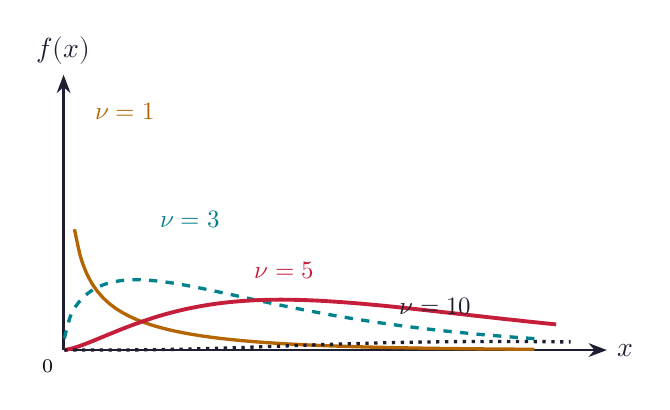
\begin{tikzpicture}[scale=0.92]
  \draw[arrow] (0, 0) -- (7.5, 0) node[right] {$x$};
  \draw[arrow] (0, 0) -- (0, 3.8) node[above] {$f(x)$};

  \node[below left, font=\scriptsize] at (0, 0) {$0$};

  % nu = 1 (L-shaped)
  \draw[line width=1.2pt, color=myamber, domain=0.15:6.5, samples=80, smooth]
    plot (\x, {0.7 * \x^(-0.5) * exp(-\x / 2)});
  \node[color=myamber, font=\small\bfseries, right] at (0.3, 3.3) {$\nu = 1$};

  % nu = 3 (starts at 0)
  \draw[line width=1.2pt, color=myteal, dashed, domain=0.01:6.5, samples=80, smooth]
    plot (\x, {1.6 * \x^(0.5) * exp(-\x / 2)});
  \node[color=myteal, font=\small\bfseries, right] at (1.2, 1.8) {$\nu = 3$};

  % nu = 5
  \draw[line width=1.4pt, color=myred, domain=0.01:6.8, samples=80, smooth]
    plot (\x, {0.6 * \x^(1.5) * exp(-\x / 2)});
  \node[color=myred, font=\small\bfseries, right] at (2.5, 1.1) {$\nu = 5$};

  % nu = 10
  \draw[line width=1.2pt, color=mydark, dotted, domain=0.01:7, samples=80, smooth]
    plot (\x, {0.005 * \x^4 * exp(-\x / 1.5)});
  \node[color=mydark, font=\small\bfseries, right] at (4.5, 0.6) {$\nu = 10$};
\end{tikzpicture}
\end{tcolorbox}

\newpage
% ===============================================================================
\section{Chi-Square Test of Goodness of Fit}
% ===============================================================================

\subsection{Principle and Pearson's Test Statistic}

\begin{tcolorbox}[defbox, title={\textbf{Pearson's Chi-Square Goodness of Fit}}]
The goodness of fit test evaluates whether an observed frequency distribution conforms to a theoretical probability distribution (such as Binomial, Poisson, or Normal). Let:
\begin{itemize}[leftmargin=12pt, itemsep=2pt]
  \item $O_i$ = Observed frequency in the $i$-th class ($i = 1, 2, \ldots, k$).
  \item $E_i$ = Expected frequency under theoretical model, with $\sum_{i=1}^k E_i = \sum_{i=1}^k O_i = N$.
\end{itemize}
Karl Pearson proved that the test statistic:
\begin{equation}
  \chi^2 = \sum_{i=1}^k \frac{(O_i - E_i)^2}{E_i} = \sum_{i=1}^k \frac{O_i^2}{E_i} - N
\end{equation}
asymptotically follows a Chi-square distribution with $\nu$ degrees of freedom:
\begin{equation}
  \nu = k - 1 - m
\end{equation}
where $k$ is the number of classes after pooling, and $m$ is the number of independent population parameters estimated from the sample data.
\end{tcolorbox}

\begin{tcolorbox}[formulabox, title={\textbf{Conditions for Validity of $\chi^2$ Test}}]
To ensure accurate approximation of discrete multinomial probabilities by continuous $\chi^2$:
\begin{enumerate}[leftmargin=14pt, itemsep=2pt]
  \item \textbf{Total Sample Size:} $N = \sum O_i \ge 50$.
  \item \textbf{Minimum Expected Frequency:} Each $E_i \ge 5$. If any $E_i < 5$, it must be \textbf{pooled (combined)} with adjacent classes, reducing $k$.
  \item \textbf{Independent Observations:} Sampling units must be mutually independent.
  \item \textbf{Linear Constraint:} $\sum O_i = \sum E_i = N$, which consumes 1 degree of freedom.
\end{enumerate}
\end{tcolorbox}

\begin{tcolorbox}[examplebox, title={\textbf{Worked Example: Chi-Square Test of Goodness of Fit}}]
A die is rolled 120 times, yielding the following face frequencies: 15, 23, 18, 16, 26, 22. Test at the 5\% level whether the die is fair ($\chi^2_{0.05, 5} = 11.07$).

\textbf{Solution:}
\begin{enumerate}[leftmargin=14pt, itemsep=2pt]
  \item \textbf{Hypotheses:} $H_0$: The die is fair ($p_i = 1/6$) vs. $H_1$: The die is biased.
  \item \textbf{Expected Frequencies:} $E_i = 120 \times \frac{1}{6} = 20$ for all $i = 1, \ldots, 6$. All $E_i \ge 5$.
  \item \textbf{Computation Table:}
\end{enumerate}
\par\vspace{2pt}\noindent
\begin{tabularx}{\linewidth}{*{5}{>{\small\centering\arraybackslash}X}}
\toprule
\textbf{Face ($i$)} & \textbf{Observed ($O_i$)} & \textbf{Expected ($E_i$)} & $O_i - E_i$ & $(O_i - E_i)^2 / E_i$ \\
\midrule
1 & 15 & 20 & $-5$ & $25 / 20 = 1.25$ \\
2 & 23 & 20 & $+3$ & $9 / 20 = 0.45$ \\
3 & 18 & 20 & $-2$ & $4 / 20 = 0.20$ \\
4 & 16 & 20 & $-4$ & $16 / 20 = 0.80$ \\
5 & 26 & 20 & $+6$ & $36 / 20 = 1.80$ \\
6 & 22 & 20 & $+2$ & $4 / 20 = 0.20$ \\
\midrule
\textbf{Total} & \textbf{120} & \textbf{120} & \textbf{0} & $\mathbf{\chi^2_{\text{cal}} = 4.70}$ \\
\bottomrule
\end{tabularx}
\par\vspace{4pt}
\textbf{Decision:} With $\nu = 6 - 1 = 5$ d.f., $\chi^2_{\text{crit}} = 11.07$. Since $\chi^2_{\text{cal}} = 4.70 < 11.07$, we fail to reject $H_0$. The die is consistent with being unbiased.
\end{tcolorbox}

\newpage
% ===============================================================================
\section{Chi-Square Test for Independence of Attributes}
% ===============================================================================

\subsection{\texorpdfstring{$r \times c$}{r x c} Contingency Tables}

\begin{tcolorbox}[defbox, title={\textbf{Contingency Table and Expected Cell Frequency}}]
When $N$ observations are classified simultaneously across two qualitative attributes $A$ (with $r$ levels $A_1, \ldots, A_r$) and $B$ (with $c$ levels $B_1, \ldots, B_c$), the frequencies form an $r \times c$ contingency table.

\textbf{Null Hypothesis:} $H_0$: Attributes $A$ and $B$ are independent.

Under $H_0$, $P(A_i \cap B_j) = P(A_i)P(B_j)$, yielding the \textbf{expected cell frequency} $E_{ij}$:
\begin{equation}
  E_{ij} = N \times \left(\frac{R_i}{N}\right) \times \left(\frac{C_j}{N}\right) = \frac{R_i \times C_j}{N}
\end{equation}
where $R_i$ is the $i$-th row total, $C_j$ is the $j$-th column total, and $N$ is the grand total.
The test statistic is:
\begin{equation}
  \chi^2 = \sum_{i=1}^r \sum_{j=1}^c \frac{(O_{ij} - E_{ij})^2}{E_{ij}}
\end{equation}
with degrees of freedom:
\begin{equation}
  \nu = (r - 1)(c - 1)
\end{equation}
\end{tcolorbox}

\subsection{\texorpdfstring{$2 \times 2$}{2 x 2} Contingency Table and Yates' Continuity Correction}

\begin{tcolorbox}[formulabox, title={\textbf{$2 \times 2$ Contingency Table Formula}}]
For a $2 \times 2$ contingency table with counts:
\par\vspace{2pt}\noindent
\begin{center}
\begin{tabular}{c c c c}
\toprule
 & $B_1$ & $B_2$ & \textbf{Total} \\
\midrule
$A_1$ & $a$ & $b$ & $a + b$ \\
$A_2$ & $c$ & $d$ & $c + d$ \\
\midrule
\textbf{Total} & $a + c$ & $b + d$ & $N = a + b + c + d$ \\
\bottomrule
\end{tabular}
\end{center}
\par\vspace{2pt}
The standard chi-square statistic ($\nu = (2-1)(2-1) = 1$) simplifies algebraically to:
\begin{equation}
  \chi^2 = \frac{N (ad - bc)^2}{(a + b)(c + d)(a + c)(b + d)}
\end{equation}

\textbf{Yates' Correction for Continuity:}
Because $\chi^2$ is continuous while counts $a, b, c, d$ are discrete integers, Frank Yates introduced a correction when $\nu = 1$ and any cell frequency is small ($< 5$):
\begin{equation}
  \chi_{\text{corr}}^2 = \frac{N \left(|ad - bc| - \dfrac{N}{2}\right)^2}{(a + b)(c + d)(a + c)(b + d)}
\end{equation}
This continuity correction reduces $\chi^2_{\text{cal}}$, preventing inflated Type I error rates.
\end{tcolorbox}

\newpage
% ===============================================================================
% QUICK REVISION SPREAD (MANDATORY 3-PAGE SPREAD)
% ===============================================================================

% ─── QUICK REVISION PAGE 1 OF 3: Formulas & Definitions ────────────────────────
\begin{center}
  {\large\bfseries\color{myred} Quick Revision --- Module 6}\\[1pt]
  {\small\color{mydark} Small Samples: $t$-Test, $F$-Test, and Chi-Square Distribution $|$ BS-M301}
\end{center}
\noindent{\color{myred}\rule{\linewidth}{1.0pt}}
\vspace{1pt}

\begin{tcolorbox}[formulabox, top=2pt, bottom=2pt, title={\textbf{Key Small Sample and Chi-Square Formulas at a Glance}}]
\renewcommand{\arraystretch}{0.94}
\setlength{\tabcolsep}{3.5pt}
\begin{tabularx}{\linewidth}{B{3.8cm} X}
Single Mean $t$-Test & $t = \frac{\bar{x} - \mu_0}{s / \sqrt{n}}, \quad s^2 = \frac{1}{n-1}\sum (x_i - \bar{x})^2, \quad \nu = n - 1$ \\[0.2pt]
Two-Sample Mean $t$-Test & $t = \frac{\bar{x}_1 - \bar{x}_2}{s_p\sqrt{1/n_1 + 1/n_2}}, \quad s_p^2 = \frac{(n_1-1)s_1^2 + (n_2-1)s_2^2}{n_1+n_2-2}, \quad \nu = n_1 + n_2 - 2$ \\[0.2pt]
Paired $t$-Test & $t = \frac{\bar{d}}{s_d / \sqrt{n}}, \quad d_i = x_i - y_i, \quad s_d^2 = \frac{1}{n-1}\sum (d_i - \bar{d})^2, \quad \nu = n - 1$ \\[0.2pt]
Correlation $t$-Test & $t = \frac{r\sqrt{n-2}}{\sqrt{1-r^2}}, \quad \nu = n - 2$ \\[0.2pt]
Fisher's $F$-Statistic & $F = \frac{s_1^2}{s_2^2} \ge 1, \quad \nu_1 = n_1 - 1, \quad \nu_2 = n_2 - 1$ \\[0.2pt]
$\chi^2$ Goodness of Fit & $\chi^2 = \sum_{i=1}^k \frac{(O_i - E_i)^2}{E_i}, \quad \nu = k - 1 - m$ \\[0.2pt]
$2 \times 2$ Contingency $\chi^2$ & $\chi^2 = \frac{N(ad - bc)^2}{(a+b)(c+d)(a+c)(b+d)}, \quad \nu = 1$ \\[0.2pt]
Yates' Correction & $\chi_{\text{corr}}^2 = \frac{N\left(|ad - bc| - N/2\right)^2}{(a+b)(c+d)(a+c)(b+d)}$ \\
\end{tabularx}
\end{tcolorbox}

\vspace{-2pt}

\begin{tcolorbox}[defbox, top=2pt, bottom=2pt, title={\textbf{One-Line Definitions}}]
\small
\begin{itemize}[leftmargin=11pt, itemsep=-0.6pt, topsep=0pt]
  \item \textbf{Small Sample:} A statistical sample with size $n < 30$, requiring exact distributions ($t, F, \chi^2$) rather than the standard normal $Z$-test.
  \item \textbf{Degrees of Freedom ($\nu$):} The number of unconstrained, freely variable observations used in evaluating a sample statistic ($\nu = n - k$).
  \item \textbf{Student's $t$-Distribution:} The exact distribution of the ratio of a standard normal variable to the square root of an independent $\chi^2$ variable divided by its d.f.
  \item \textbf{Pooled Variance ($s_p^2$):} The weighted average of two independent sample variances used in two-sample $t$-tests under equal population variances.
  \item \textbf{Paired $t$-Test:} A test applied to dependent matched pairs where differences $d_i = x_i - y_i$ eliminate extraneous subject variability.
  \item \textbf{Snedecor's $F$-Distribution:} The distribution of the ratio of two independent chi-square variables, each divided by its d.f. ($s_1^2 / s_2^2$).
  \item \textbf{Chi-Square ($\chi^2$) Distribution:} The distribution formed by the sum of squares of $\nu$ independent standard normal random variables.
  \item \textbf{Goodness of Fit:} A statistical test measuring whether an empirical sample frequency distribution adheres to a theoretical distribution.
  \item \textbf{Contingency Table:} A grid matrix displaying the bivariate joint frequency distribution of two qualitative attributes.
  \item \textbf{Yates' Correction:} A continuity correction subtracting $N/2$ from $|ad - bc|$ in $2 \times 2$ tables to account for discrete counts in continuous $\chi^2$.
\end{itemize}
\end{tcolorbox}

\newpage
% ─── QUICK REVISION PAGE 2 OF 3: Viva Q&A Part 1 ───────────────────────────────
\begin{tcolorbox}[exambox, title={\textbf{Frequently Asked / Viva Questions (Part 1)}}]
\small
\begin{enumerate}[leftmargin=14pt, itemsep=3pt]
\item \Q{Q1. Why can we not use the standard normal $Z$-test for small samples ($n < 30$)?}
For $n < 30$, the Central Limit Theorem cannot guarantee normality of the sampling distribution unless the parent population is normal. Furthermore, substituting the sample variance $s^2$ for the unknown $\sigma^2$ introduces substantial additional sampling variability, making the tails of the distribution much heavier than $N(0, 1)$. Gosset's $t$-distribution accounts precisely for this extra variability.

\item \Q{Q2. What are the key assumptions underlying the two-sample independent $t$-test?}
The assumptions are: (1) both parent populations are normally distributed, (2) the two samples are selected randomly and independently, and (3) the two population variances are equal ($\sigma_1^2 = \sigma_2^2 = \sigma^2$, known as homoscedasticity). Equality of variances is checked using an $F$-test.

\item \Q{Q3. When should a paired $t$-test be used instead of an independent two-sample $t$-test?}
A paired $t$-test must be used when the two sets of observations are intrinsically dependent, such as measurements on the same physical subjects before and after a treatment, or twin studies. It isolates the treatment effect by converting paired data into single differences $d_i = x_i - y_i$, thereby eliminating between-subject biological or physical variance.

\item \Q{Q4. State the relation between Student's $t$, Snedecor's $F$, and Chi-square $\chi^2$ distributions.}
Key interrelations include:
\begin{itemize}[leftmargin=12pt, itemsep=1pt]
  \item The square of a $t$-variable with $\nu$ d.f.\ is an $F$-variable with $(1, \nu)$ d.f.: $t_\nu^2 = F_{1, \nu}$.
  \item As the denominator degrees of freedom $\nu_2 \to \infty$, $\nu_1 F_{\nu_1, \nu_2} \to \chi^2(\nu_1)$.
  \item As degrees of freedom $\nu \to \infty$, Student's $t(\nu) \to N(0, 1)$.
\end{itemize}

\item \Q{Q5. Why is the larger sample variance always placed in the numerator in an $F$-test?}
By convention, setting $F = s_1^2 / s_2^2$ with $s_1^2 \ge s_2^2$ ensures $F \ge 1$. This allows the use of standard upper-tail $F$-distribution critical value tables without needing to invert lower-tail critical values ($F_{1-\alpha} = 1 / F_\alpha$).

\item \Q{Q6. What are the fundamental validity conditions for Karl Pearson's Chi-square test?}
The conditions are: (1) total sample size $N = \sum O_i \ge 50$, (2) each theoretical expected frequency $E_i \ge 5$ (if $E_i < 5$, adjacent cells must be pooled), (3) individual observations are drawn randomly and independently, and (4) $\sum O_i = \sum E_i = N$.

\item \Q{Q7. How are degrees of freedom calculated in an $r \times c$ contingency table?}
The degrees of freedom are $\nu = (r - 1)(c - 1)$. This arises because the marginal row totals impose $r$ constraints and the column totals impose $c$ constraints, with one common grand total constraint $N$, leaving $(r-1)(c-1)$ independently assignable cells.
\end{enumerate}
\end{tcolorbox}

\newpage
% ─── QUICK REVISION PAGE 3 OF 3: Viva Q&A Part 2 & Summary Comparison Matrix ───
\begin{tcolorbox}[exambox, title={\textbf{Frequently Asked / Viva Questions (Part 2)}}]
\small
\begin{enumerate}[leftmargin=14pt, itemsep=3pt]
\setcounter{enumi}{7}
\item \Q{Q8. What is Yates' correction for continuity and when is it mandatory?}
Yates' correction adjusts the discrete cell counts in a $2 \times 2$ table to match the continuous theoretical $\chi^2$ density by subtracting $N/2$ from the absolute difference $|ad - bc|$. It is mandatory when $\nu = 1$ and any cell frequency is less than 5 ($E_{ij} < 5$), preventing spurious rejections of $H_0$.

\item \Q{Q9. How do you test whether an observed sample correlation coefficient $r = 0.6$ from $n = 18$ pairs is statistically significant?}
We test $H_0: \rho = 0$ using $t = \frac{r\sqrt{n-2}}{\sqrt{1-r^2}} = \frac{0.6\sqrt{16}}{\sqrt{1 - 0.36}} = \frac{0.6 \times 4}{0.8} = 3.00$. With $\nu = 18 - 2 = 16$ d.f., the critical value at $\alpha = 0.05$ is $t_{0.025, 16} = 2.12$. Since $|t_{\text{cal}}| = 3.00 > 2.12$, the correlation is statistically significant.

\item \Q{Q10. What does a non-significant result in a $\chi^2$ goodness-of-fit test signify?}
When $\chi^2_{\text{cal}} \le \chi^2_{\text{crit}}$, we fail to reject $H_0$. This indicates that the observed sampling discrepancies from theoretical frequencies are small enough to be attributed purely to chance, confirming the theoretical model fits the empirical data well.
\end{enumerate}
\end{tcolorbox}

\vspace{-2pt}

\begin{tcolorbox}[tikzbox, top=2pt, bottom=2pt, title={\textbf{Summary Matrix: Comparison of Small Sample Tests ($t$, $F$, $\chi^2$)}}]
\renewcommand{\arraystretch}{0.96}
\setlength{\tabcolsep}{3.5pt}
\par\vspace{1pt}\noindent
\begin{tabularx}{\linewidth}{B{2.3cm} B{2.5cm} Y >{\small\centering\arraybackslash}X}
\toprule
\textbf{Test} & \textbf{Objective} & \textbf{Test Statistic \& Parameters} & \textbf{d.f. ($\nu$)} \\
\midrule
Single Mean $t$ & Test $H_0: \mu = \mu_0$ ($\sigma$ unknown) & $t = \dfrac{\bar{x} - \mu_0}{s / \sqrt{n}}, \quad s^2 = \dfrac{\sum(x_i - \bar{x})^2}{n - 1}$ & $n - 1$ \\
Two-Sample $t$ & Compare two means ($\sigma_1 = \sigma_2$) & $t = \dfrac{\bar{x}_1 - \bar{x}_2}{s_p\sqrt{1/n_1 + 1/n_2}}$, pooled $s_p^2$ & $n_1 + n_2 - 2$ \\
Paired $t$ & Before vs. After on same units & $t = \dfrac{\bar{d}}{s_d / \sqrt{n}}$, differences $d_i = x_i - y_i$ & $n - 1$ \\
Correlation $t$ & Test $H_0: \rho = 0$ & $t = \dfrac{r\sqrt{n-2}}{\sqrt{1 - r^2}}$ & $n - 2$ \\
Fisher's $F$ & Compare $\sigma_1^2$ vs $\sigma_2^2$ & $F = \dfrac{s_1^2}{s_2^2}$ ($s_1^2 \ge s_2^2$) & $(n_1 - 1, n_2 - 1)$ \\
Pearson's $\chi^2$ & Goodness of Fit & $\chi^2 = \sum \dfrac{(O_i - E_i)^2}{E_i}$ & $k - 1 - m$ \\
Contingency $\chi^2$ & Independence of attributes & $\chi^2 = \sum \sum \dfrac{(O_{ij} - E_{ij})^2}{E_{ij}}$ or $2 \times 2$ Yates & $(r - 1)(c - 1)$ \\
\bottomrule
\end{tabularx}
\end{tcolorbox}

\end{document}
